% =====================================================================
%  ASTRO-NOT  --  practical report template
%  Mapping the Milky Way's rotation curve with the 21 cm line (HI4PI)
%
%  HOW TO USE THIS FILE
%  --------------------
%  1. Compile with pdfLaTeX. On Overleaf: Menu > Compiler > pdfLaTeX.
%     Run it twice, then once more after the bibliography changes.
%  2. Fill in every \ph{...} marker and then delete the marker itself.
%     Nothing grey should survive into the version you hand in.
%  3. The lines beginning with % are notes for you. They do not appear
%     in the PDF. Delete them or leave them, as you prefer.
%  4. Write the prose yourself. Where a paragraph is already written
%     here it is there to set the register, not to be handed back to us
%     unchanged. A report that reads like this template will be marked
%     as a report that was not written.
%  5. Keep the section order. It is the order a reader needs the
%     information in: what the problem is, what the physics says, what
%     the data are, what was done to them, what came out, what it means,
%     and what could be wrong with it.
% =====================================================================
\documentclass[11pt,a4paper]{article}
\usepackage{astronot}

\renewcommand{\reportshorttitle}{Mapping the Milky Way's rotation curve}

% ---------------------------------------------------------------------
\begin{document}

\begin{titlepage}
\centering
\vspace*{2cm}

{\scshape\large Astro-Not}\\[0.3cm]
{\small A practical in observational astrophysics}\\[1.2cm]

\rule{\textwidth}{0.6pt}\\[0.6cm]
{\LARGE Mapping the Milky Way's Rotation Curve\\[0.3cm]
from the 21\,cm Line of Neutral Hydrogen}\\[0.6cm]
\rule{\textwidth}{0.6pt}\\[0.8cm]

{\large A tangent-point analysis of the HI4PI all-sky survey}\\[2cm]

{\large \ph{Your name}}\\[0.3cm]
{\ph{Your institution or school}}\\[0.3cm]
{\small \ph{your.email@example.com}}\\[2cm]

{\ph{Date of submission}}

\vfill
{\small Practical supervised by Astro-Not.\\
Data: HI4PI Collaboration (2016). Constants: Reid et al. (2019).}
\end{titlepage}
\setcounter{page}{2}   % the title page is page 1 and carries no number

% ---------------------------------------------------------------------
\begin{abstract}
\noindent
% Write the abstract LAST, once you know what your numbers are.
% It must contain: what was measured, from what data, by what method,
% the result with an uncertainty, and the dominant systematic. Roughly
% 150-200 words, no citations, no equations.
The circular-speed curve of the inner Milky Way is measured from the 21\,cm
line of neutral hydrogen by the tangent-point method. Spectra were taken
from the HI4PI all-sky survey, averaged over the latitude strip
$|b| \le 0.5\degr$ and binned to \ph{bin} in Galactic longitude over the range
\ph{$l_{\min}$}$\,\le l \le\,$\ph{$l_{\max}$}. Terminal velocities were
extracted with a fixed brightness threshold $\Tthr = \ph{value}$\,K and
converted to circular speeds at $R = \Rzero|\sin l|$, adopting
$\Rzero = 8.15$\,\kpc\ and $\Tzero = 236$\,\kms. The measured curve
\ph{describe the shape in one clause: rise, plateau, value}, and the
enclosed dynamical mass within the solar circle follows as
$M(<\Rzero) = \ph{value}\times 10^{11}\,\Msun$ under a spherical
approximation. The largest single uncertainty is the definition of the
velocity edge, which is estimated here at \ph{value}\,\kms; the vanishing
of the terminal velocity as $l \to 90\degr$ is used to test for a residual
systematic offset. \ph{One closing sentence on what the curve does and does
not establish.}
\end{abstract}

\vspace{0.5cm}
\tableofcontents
\newpage

% =====================================================================
\section{Introduction}
\label{sec:intro}
% Three short paragraphs are enough.
%  (a) the problem: we are inside the thing we are trying to measure;
%  (b) why the measurement is worth making: a curve is a mass;
%  (c) what this report contains, in the order it contains it.
% Cite the survey and the constants here, not in the abstract.

Every photograph of a spiral galaxy is a photograph of somebody else's
galaxy. The Milky Way is the one disk we cannot step outside of, and
everything known about its shape has been assembled from a single
viewpoint embedded within it. A spectrum taken from that viewpoint returns
one number, the velocity of the emitting gas along the line of sight, and
it returns that number without saying how far away the gas was. The
rotation curve $\Theta(R)$ --- the circular speed of material on a circular
orbit at Galactocentric radius $R$ --- is therefore not directly observable
in the way it is for an external galaxy.

\ph{Second paragraph: say what a rotation curve buys you. Newton's shell
theorem, the mass that follows from a circular orbit, and the three
reference behaviours (Keplerian, solid-body, flat) that a measured curve
is read against. Two or three sentences.}

\ph{Third paragraph: state what this report does. Which survey, which
longitude range, which method, and what is claimed at the end of it. Be
explicit that the tangent-point method reaches only to $R = \Rzero$ and that
this bounds the conclusion.}

% =====================================================================
\section{Theory}
\label{sec:theory}

\subsection{The 21\,cm line}
\label{sec:21cm}

The ground state of atomic hydrogen is split by the interaction between the
magnetic moments of the proton and the electron. The parallel and
antiparallel spin arrangements differ slightly in energy, and the
transition between them emits a photon of that difference,
%
\begin{equation}
\Delta E = h\nu_{0} \simeq 5.874\times10^{-6}\ \mathrm{eV},
\qquad
\nu_{0} = 1420.405752\ \mathrm{MHz},
\qquad
\lambda_{0} = \frac{c}{\nu_{0}} = 21.106\ \mathrm{cm}.
\label{eq:hyperfine}
\end{equation}
%
The transition is forbidden to first order and a single atom waits some ten
million years to make it, but a sightline through the disk contains enough
hydrogen for the summed emission to be easy to detect. Three properties
make the line the right ruler for this measurement: the rest frequency is
known to better than one part in $10^{11}$, the emitting gas is present
throughout the disk, and at 21\,cm the dust that makes the Galactic plane
opaque at optical wavelengths is transparent.

\ph{Add a sentence on what a radio telescope actually records: intensity
converted to a brightness temperature in the Rayleigh--Jeans limit, and a
frequency converted to a radial velocity in the non-relativistic radio
convention. State which velocity frame your data arrive in.}

\subsection{Differential rotation along a sightline}
\label{sec:diffrot}

Let $C$ be the Galactic Centre, $S$ the Sun and $P$ a hydrogen cloud at
Galactocentric radius $R$ on a sightline of Galactic longitude $l$. Taking
both the Sun and the gas to move on circular orbits, each velocity vector is
perpendicular to its own radius vector, and the sine rule in the triangle
$CSP$ gives $\sin\gamma = (\Rzero/R)\sin l$ for the angle $\gamma$ at $P$.
Projecting both velocities onto the sightline and subtracting the solar
contribution,
%
\begin{equation}
\vlsr(l,R) = \left[\Theta(R)\frac{\Rzero}{R} - \Tzero\right]\sin l
           = \Rzero\left[\Omega(R) - \Omega_{0}\right]\sin l .
\label{eq:vlsr}
\end{equation}
%
Equation~\eqref{eq:vlsr} vanishes identically if $\Omega(R) = \Omega_{0}$
everywhere. A rigidly rotating Galaxy would betray no rotation at all,
however fast it spun: what the 21\,cm line measures is differential
rotation.

\subsection{The tangent point}
\label{sec:tangent}

Along one sightline the Galactocentric radius of a point at heliocentric
distance $d$ follows from the cosine rule, $R^{2}(d) = \Rzero^{2} + d^{2} -
2\Rzero d\cos l$. Minimising with respect to $d$,
%
\begin{equation}
\dtan = \Rzero\cos l
\qquad\Longrightarrow\qquad
\Rtan = \Rzero\,|\sin l| ,
\label{eq:rtan}
\end{equation}
%
with second derivative $+2 > 0$, confirming a minimum. At that point the
radius vector is perpendicular to the sightline, so the orbital velocity
lies exactly along it and the full circular speed appears in the Doppler
shift. No distance has been measured: the radius follows from the longitude
alone, and that is the step which makes the method work.

Provided $\mathrm{d}\Omega/\mathrm{d}R < 0$, the tangent point also carries
the largest radial velocity on the sightline. The extreme velocity at which
\HI\ is still seen is the terminal velocity \vterm. Evaluating
equation~\eqref{eq:vlsr} at $R = \Rtan$ gives the pair of results the whole
analysis is built on,
%
\begin{equation}
\boxed{\;\Theta(R) = |\vterm| + \Tzero|\sin l|
\qquad\text{at}\qquad
R = \Rzero|\sin l| \;}
\label{eq:master}
\end{equation}
%
The absolute values carry the same expressions into Quadrant IV, where
$\sin l$ and \vterm\ are both negative.

\subsection{The curve as a mass}
\label{sec:mass}

For a spherically symmetric mass distribution, Newton's shell theorem lets
the gravitational and centripetal accelerations of a circular orbit be
equated directly,
%
\begin{equation}
\frac{GM(<R)}{R^{2}} = \frac{\Theta^{2}(R)}{R}
\qquad\Longrightarrow\qquad
M(<R) = \frac{\Theta^{2}(R)\,R}{G} .
\label{eq:mass}
\end{equation}
%
The orbiting body's own mass cancels, which is why hydrogen serves as a
tracer without any of its own properties entering the result. If the curve
is flat then $M(<R) \propto R$, and comparison with the spherical mass
integral gives $\rho(R) \propto R^{-2}$.

% Note for you: equation (5) is exact only for spherical symmetry. The
% disk is flattened, so Theta^2 R / G is a dynamical mass scale rather
% than a precision mass. Say so where you quote a mass, not here.

% =====================================================================
\section{Data}
\label{sec:data}

HI4PI is a full-sky \HI\ survey merging EBHIS, from the Effelsberg 100\,m
telescope, with GASS, from the Parkes 64\,m \citep{hi4pi2016}. The merged
product has an angular resolution of $16.2'$, a velocity-channel width of
1.29\,\kms\ and a channel noise near 43\,mK. The data form a
three-dimensional cube $\TB(v,b,l)$: one spectrum for every direction on
the sky. Averaging over a thin strip in latitude collapses the cube into a
longitude--velocity diagram, $\TB(v,l)$, whose upper velocity envelope is
the terminal-velocity curve.

The constants in Table~\ref{tab:constants} are not measured here. They set
the radius scale and the velocity zero-point of every point on the final
curve, and a curve quoted without them cannot be compared with anybody
else's.

\begin{table}[htbp]
\centering
\caption{Constants adopted in this analysis.}
\label{tab:constants}
\begin{tabular}{llll}
\toprule
Quantity & Symbol & Value & Source \\
\midrule
\HI\ rest frequency      & $\nu_{0}$ & 1420.405752\,MHz & atomic physics \\
\HI\ rest wavelength     & $\lambda_{0}$ & 21.106\,cm & $\lambda_{0}=c/\nu_{0}$ \\
Sun--Centre distance     & \Rzero & $8.15 \pm 0.15$\,\kpc & \citet{reid2019} \\
Local circular speed     & \Tzero & $236 \pm 7$\,\kms & \citet{reid2019} \\
Gravitational constant   & $G$ & $4.30091\times10^{-6}$\,kpc\,(\kms)$^{2}\,\Msun^{-1}$ & converted units \\
\bottomrule
\end{tabular}
\end{table}

\paragraph{Cuts applied.}
% State each cut and the reason for it. The reasons are physical, not
% cosmetic, and a reader will ask for them.
\begin{itemize}\itemsep2pt
  \item Latitude: $|b| \le 0.5\degr$. \ph{Why: the geometry assumes gas in
        the midplane, and half a degree at a tangent-point distance of
        7\,kpc is only about 60\,pc. Put this in your own words and check
        the arithmetic.}
  \item Longitude: \ph{range used}. \ph{Why bounded below --- the bar and
        non-circular motions inside $R \approx 2$\,kpc --- and why bounded
        above --- the terminal velocity falls below the line broadening.}
  \item Longitude binning: \ph{bin size}. \ph{Why: sightlines closer
        together than the $16.2'$ beam are not independent measurements.}
\end{itemize}

% =====================================================================
\section{Method}
\label{sec:method}

\subsection{Locating the velocity edge}
\label{sec:edge}

A real 21\,cm spectrum is a landscape of peaks, because the sightline
crosses many clouds at many distances. The height of a peak records how
much gas emits at that velocity, not how fast anything moves; the
tangent-point information sits entirely in the extreme-velocity edge, and
the way that edge is defined governs the result \citep{mcclure2007}.
Figure~\ref{fig:spectrum} shows one spectrum with the edge criterion
applied.

The edge was defined by a fixed brightness threshold
$\Tthr = \ph{value}$\,K, applied identically at every longitude, together
with two further rules: \ph{state your consecutive-channel rule, and state
whether the crossing was interpolated between channels or rounded to a
channel boundary}. A fixed threshold is preferable to a fixed fraction of
the local peak, because peak brightness and the identity of the tallest
peak both vary from sightline to sightline, so a fractional criterion
silently applies a different physical definition at every longitude.

\begin{figure}[htbp]
\centering
% Replace this file with your own spectrum. Keep the width; keep the
% axis labels in km/s and K; keep the threshold marked.
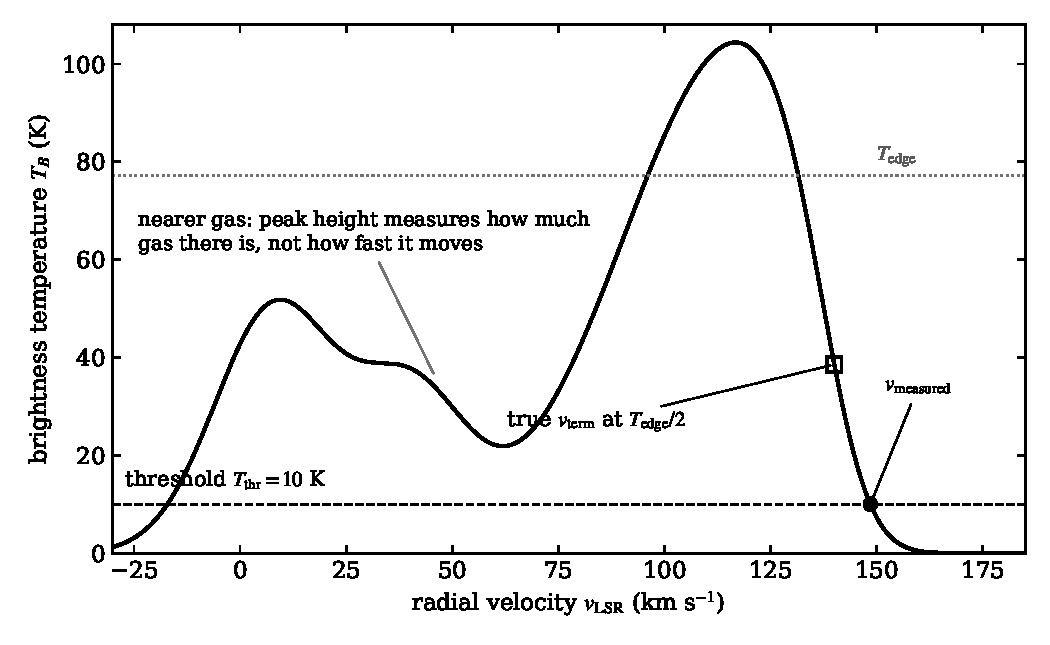
\includegraphics[width=0.82\textwidth]{sample_spectrum}
\caption{A 21\,cm spectrum along a single sightline, with the edge
criterion marked. The measurement is the position of the high-velocity
edge, not the position or height of the brightest peak. A fixed brightness
threshold locates the edge consistently from sightline to sightline, but
lands a little outside the true terminal velocity, which sits at the
half-power point of the falling edge.
\ph{Replace with your own sightline and state its longitude here.}}
\label{fig:spectrum}
\end{figure}

\subsection{The bias in the edge}
\label{sec:bias}

The edge is not a cliff. Thermal and turbulent motions give the gas a
velocity dispersion of $\sigma \approx 8$--$10$\,\kms, and the finite beam
averages a patch of sky across which the terminal velocity varies.
Convolving an intrinsically sharp edge with a Gaussian of dispersion
$\sigma$ returns a complementary error function, so that the true terminal
velocity lies at the half-power point $\Tedge/2$ of the falling edge, and
the threshold crossing sits at
%
\begin{equation}
v_{\mathrm{measured}} - \vterm
= \sqrt{2}\,\sigma\;\mathrm{erfc}^{-1}\!\left(\frac{2\Tthr}{\Tedge}\right).
\label{eq:bias}
\end{equation}
%
\ph{Evaluate equation~(\ref{eq:bias}) for your own $\Tthr$, your typical
\Tedge\ and an assumed $\sigma$, and quote the bias in \kms. State whether
you corrected for it or carried it as a systematic.}

\subsection{The test at high longitude}
\label{sec:test}

There is one place in the sky where the answer is known in advance. As
$l \to 90\degr$ the tangent point approaches the Sun's own orbit,
$\Rtan \to \Rzero$, so $\Theta(\Rtan) \to \Tzero$ and the terminal velocity
must fall to zero. Expanding $\Theta$ about \Rzero\ to first order,
%
\begin{equation}
v_{\mathrm{term}}^{\,\mathrm{ideal}}(l)
= \left[\Tzero - \Rzero\Theta'(\Rzero)\right](1 - \sin l)
= 2A\Rzero\,(1 - \sin l),
\label{eq:ideal}
\end{equation}
%
where $A$ is Oort's constant. Any persistent excess measured at high
longitude is therefore a systematic, whether it comes from the edge
definition, from the velocity frame, or from both.

\ph{Report what your own high-longitude points give against
equation~(\ref{eq:ideal}), and what you did about the difference.}

% =====================================================================
\section{Results}
\label{sec:results}

\subsection{A single sightline}
\label{sec:worked}

% Work one longitude through by hand, in full, before showing the whole
% curve. It proves the chain works and it lets a reader check your
% arithmetic against their own.

At $l = \ph{value}\degr$ the measured terminal velocity is
$\vterm = \ph{value}$\,\kms. Equation~\eqref{eq:rtan} places this at
$R = \ph{value}$\,\kpc, equation~\eqref{eq:master} gives
$\Theta = \ph{value}$\,\kms, and equation~\eqref{eq:mass} gives
$M(<R) = \ph{value}\times10^{10}\,\Msun$. Propagating
$\delta\vterm$, $\delta\Tzero$ and $\delta\Rzero$ as in
Appendix~\ref{app:errors}, $\delta\Theta = \ph{value}$\,\kms\ and
$\delta M/M = \ph{value}$.

\subsection{The rotation curve}
\label{sec:curve}

\ph{Describe the curve you obtained: where it rises, where it flattens, what
range of $\Theta$ the plateau occupies, and how far out in radius the
measurement reaches. Refer to your figure. Say something about the
wiggles --- with a channel noise of 43\,mK against a 10\,K threshold,
receiver noise is not what produces them.}

% A second figure goes here once you have one: the rotation curve itself,
% with error bars, and the three reference behaviours drawn for comparison.
% Copy the figure environment above and change the file name and caption.

\begin{table}[htbp]
\centering
\caption{Extracted tangent-point measurements. Add or remove rows as
needed; a long table belongs in an appendix, not here.}
\label{tab:results}
\begin{tabular}{cccccc}
\toprule
$l$ (\degr) & \vterm\ (\kms) & $R$ (\kpc) & $\Theta$ (\kms)
& $\delta\Theta$ (\kms) & $M(<R)$ ($10^{10}\,\Msun$) \\
\midrule
\ph{ } & \ph{ } & \ph{ } & \ph{ } & \ph{ } & \ph{ } \\
\ph{ } & \ph{ } & \ph{ } & \ph{ } & \ph{ } & \ph{ } \\
\ph{ } & \ph{ } & \ph{ } & \ph{ } & \ph{ } & \ph{ } \\
\bottomrule
\end{tabular}
\end{table}

\subsection{The enclosed mass}
\label{sec:massresult}

At the Sun's own radius, equation~\eqref{eq:mass} with the adopted \Tzero\
gives
%
\begin{equation}
M(<\Rzero) \simeq \frac{(236)^{2}\times 8.15}{4.30091\times10^{-6}}
\simeq 1.06\times10^{11}\,\Msun .
\label{eq:msun}
\end{equation}
%
\ph{Quote your own value and its uncertainty here, and compare it with
equation~(\ref{eq:msun}). Then state plainly that this is a total
gravitating mass under a spherical approximation, not a dark-matter mass:
stars, gas and bulge all contribute to it, and inside the solar circle they
contribute a great deal of it.}

% =====================================================================
\section{Discussion}
\label{sec:discussion}

\subsection{What the measurement supports}

\ph{One paragraph. The defensible conclusion is that the inner Galaxy has
an extended gravitating mass distribution whose rotation is nothing like
the point-mass Keplerian expectation. Say why the method stops at \Rzero\
--- $\Rzero|\sin l| \le \Rzero$ is a geometric limit, not a shortage of
hydrogen --- and why the region it does reach is exactly the region where
visible matter contributes most strongly. A full dark-matter inference
needs a baryonic mass model and tracers beyond \Rzero\
\citep{eilers2019}.}

\subsection{Systematics}

\begin{table}[htbp]
\centering
\caption{Assumptions and the errors they produce.}
\label{tab:systematics}
\begin{tabular}{p{4.4cm}p{9.4cm}}
\toprule
Assumption or issue & Why it matters, and what it did here \\
\midrule
Circular gas orbits &
The bar and the spiral arms drive non-circular motions of several to
$\sim 10$\,\kms; the innermost points are the least reliable.
\ph{state which of your points you distrust} \\[4pt]
Edge definition &
Turbulence and beam smearing broaden the edge, and the threshold choice can
move \vterm\ by $\sim 10$\,\kms. Usually the largest single systematic.
\ph{your estimate} \\[4pt]
Velocity frame &
The radio and dynamical LSR differ by up to $\sim 3$\,\kms, mattering most
as $l \to 90\degr$ \citep{schonrich2010}. \ph{applied or not?} \\[4pt]
Adopted \Rzero, \Tzero &
$\pm 0.15$\,\kpc\ and $\pm 7$\,\kms\ propagate into every point of the
curve. \ph{quote the resulting spread} \\[4pt]
Spherical mass formula &
The disk is flattened, so $\Theta^{2}R/G$ overestimates the true enclosed
mass and is a dynamical scale rather than a precision measurement. \\[4pt]
\ph{add your own rows} & \ph{ } \\
\bottomrule
\end{tabular}
\end{table}

\ph{Close this section by saying where the difficulty in this experiment
actually lies. HI4PI's 0.043\,K channel noise sits more than two orders of
magnitude below a 10\,K edge criterion, so effort spent on receiver noise
is effort spent on the wrong problem.}

% =====================================================================
\section{Conclusions}
\label{sec:conclusions}

% Numbered, short, and containing numbers. No new material here.
\begin{enumerate}\itemsep2pt
  \item \ph{What was measured, over what radius range, from what data.}
  \item \ph{The shape of the curve and the value of the plateau.}
  \item \ph{The enclosed dynamical mass, with its uncertainty.}
  \item \ph{The dominant systematic, and what the high-longitude test
        showed about it.}
  \item \ph{What the result does not establish on its own.}
\end{enumerate}

% =====================================================================
\section*{Acknowledgements}
\addcontentsline{toc}{section}{Acknowledgements}

This work uses data from the HI4PI survey, a joint product of the
Effelsberg--Bonn \HI\ Survey and the Galactic All-Sky Survey.
\ph{Acknowledge anyone who helped you, and state clearly any code,
software or assistance you used.}

% =====================================================================
\bibliographystyle{plainnat}
\bibliography{refs}
\addcontentsline{toc}{section}{References}

% =====================================================================
\appendix
\section{Propagation of uncertainties}
\label{app:errors}

From equation~\eqref{eq:master}, with \vterm\ and \Tzero\ independent,
%
\begin{equation}
\delta\Theta = \sqrt{\,(\delta\vterm)^{2} + (|\sin l|\,\delta\Tzero)^{2}\,},
\qquad
\delta R = |\sin l|\,\delta\Rzero ,
\label{eq:dtheta}
\end{equation}
%
and from equation~\eqref{eq:mass}, since $M \propto \Theta^{2}R$,
%
\begin{equation}
\frac{\delta M}{M}
= \sqrt{\left(\frac{2\,\delta\Theta}{\Theta}\right)^{2}
      + \left(\frac{\delta R}{R}\right)^{2}} .
\label{eq:dm}
\end{equation}
%
\ph{Note in one sentence why this is conservative: \Rzero\ and \Tzero\ are
not independently measured but jointly constrained, with their ratio
$\Omega_{0}$ pinned down far more tightly than either separately, so adding
their errors in quadrature overstates the true spread.}

\section{Formula sheet}
\label{app:formulae}

% Keep this. It is useful to a reader and it costs half a page.
\begin{align*}
\Delta E &= h\nu_{0}, \qquad \nu_{0} = 1420.405752\ \mathrm{MHz},
           \qquad \lambda_{0} = c/\nu_{0} = 21.106\ \mathrm{cm}; \\[2pt]
\TB &= \frac{c^{2}}{2k_{B}\nu^{2}}I_{\nu}, \qquad
      v_{\mathrm{rad}} \simeq c\,\frac{\nu_{0}-\nu_{\mathrm{obs}}}{\nu_{0}}; \\[2pt]
\vlsr &= \left[\Theta(R)\frac{\Rzero}{R}-\Tzero\right]\sin l
       = \Rzero\left[\Omega(R)-\Omega_{0}\right]\sin l; \\[2pt]
\dtan &= \Rzero\cos l, \qquad \Rtan = \Rzero|\sin l|, \qquad
\Theta(R) = |\vterm| + \Tzero|\sin l|; \\[2pt]
v_{\mathrm{measured}} - \vterm &= \sqrt{2}\,\sigma\,
      \mathrm{erfc}^{-1}\!\left(\frac{2\Tthr}{\Tedge}\right), \qquad
v_{\mathrm{term}}^{\,\mathrm{ideal}} = 2A\Rzero(1-\sin l); \\[2pt]
M(<R) &= \frac{\Theta^{2}(R)R}{G}, \qquad
\Theta \approx \mathrm{const} \Rightarrow M(<R) \propto R, \qquad
\rho \propto R^{-2}.
\end{align*}

\end{document}
